\chapter{粮草先行}
\begin{introduction}
	\item 计算机选购
	\item 操作系统
	\item \texttt{IDE}安装
	\item 网站推荐
	\item 学习方法
	\item 学习心态
\end{introduction}

俗话说三军未动,粮草先行。在正式开启信奥的学习之前,我们先把准备工作做好。
\section{硬件环境准备}
首先,信奥学习是需要动手编程的,那么一台电脑是必不可少的。简单说下电脑选购的事情。若我们的电脑只用来考虑信奥学习,完全不去考虑游戏的事的话,不夸张地说,只要是台能运行起来的电脑,其实都是可以拿来用的。继承下家长淘汰下来的电脑是最省钱的方案。而如果说家里还没有电脑,要买个新的话,建议是不要去线下电脑城购买,去了$ 90\% $是被宰一顿。推荐在京东购买电脑。

而对于是购买台式机还是购买笔记本,则是看你有没有携带的需求,如果你不需要带着电脑到处跑的话,同等价位下,台式机的性能是要超过笔记本的。

对于配置的选购的话,信奥学习这块,不用去刻意追求显卡的好坏,CPU自带的核显是完全够用的,重点关注下CPU、内存和硬盘即可。
\section{软件环境准备}
\subsection{操作系统}
操作系统这块,虽然在复赛的时候,是要求在\texttt{NOI Linux 2.0}\footnote{Ubuntu 20.04的魔改版本,封装了竞赛常用的一些软件,并阉割了一部分东西。}系统上进行的,但是从初学者上手的角度来说,建议可以从Windows操作系统开始,Window10/11均可。后期,等我们对计算机的相关操作已经比较熟练了,我们再转战到\texttt{Linux}平台,计划是到算法学习阶段,我们会在\texttt{NOI Linux 2.0}下进行相关内容的学习。
\subsection{集成开发环境}
集成开发环境(Integrated Development Environment,IDE),是用于我们写C++程序的。Windows上推荐两个,一个是\texttt{Dev-C++},另一个是\texttt{Code::Blocks}。两者都能开箱即用。\texttt{Dev-C++}比较小巧,可快速地进行单文件编译运行,上手门槛较低。而\texttt{Code::Blocks}不仅仅\texttt{Windows}平台下有,在\texttt{Noi Linux 2.0} 中也有该编辑器,能更顺利的进行学习环境的迁移。

两个IDE任选一个即可,重点还是在语言与算法学习上。

\subsubsection{\texttt{Dev-C++}安装}
\textbf{软件下载地址} :\href{https://wloving.lanzouq.com/dev-cpp}{https://wloving.lanzouq.com/dev-cpp}

下载好之后双击\texttt{exe}文件。
\begin{figure}[H]
\centering
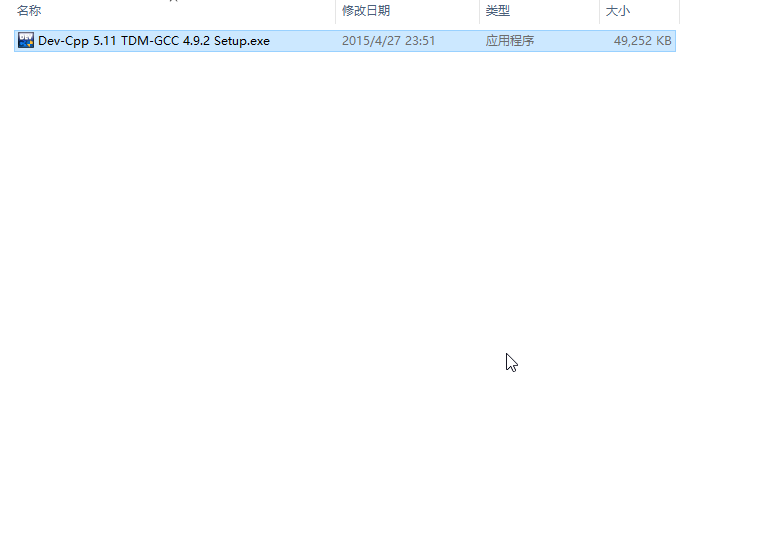
\includegraphics[width=0.6\linewidth]{01chapter/img/dev安装01}
\caption{双击安装包}
\label{fig:dev01}
\end{figure}

双击后,等待程序提取安装包内容。
\begin{figure}[H]
\centering
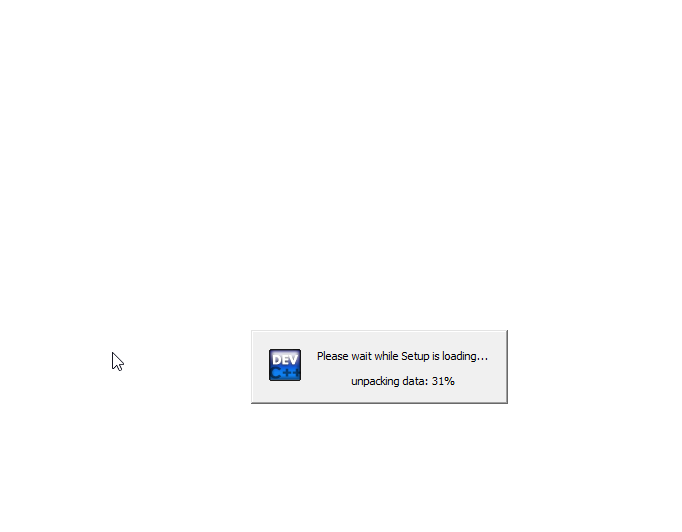
\includegraphics[width=0.6\linewidth]{01chapter/img/dev安装02}
\caption{等待提取安装包}
\label{fig:dev02}
\end{figure}
点击\texttt{I Agree},同意相关事项。
\begin{figure}[H]
\centering
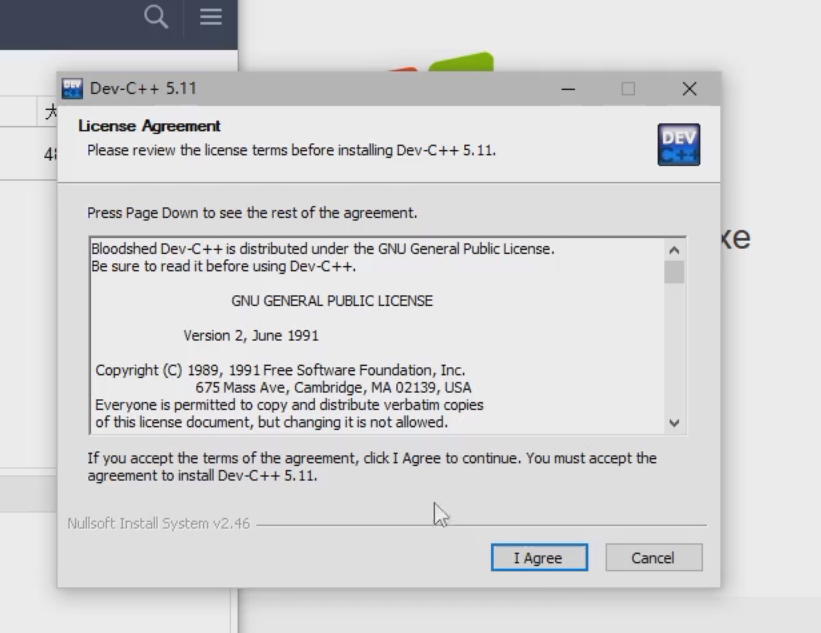
\includegraphics[width=0.6\linewidth]{01chapter/img/dev安装03}
\caption{点击同意}
\label{fig:dev03}
\end{figure}
在安装组件部分,选择默认的就行,直接点击\texttt{next}即可。
\begin{figure}[H]
\centering
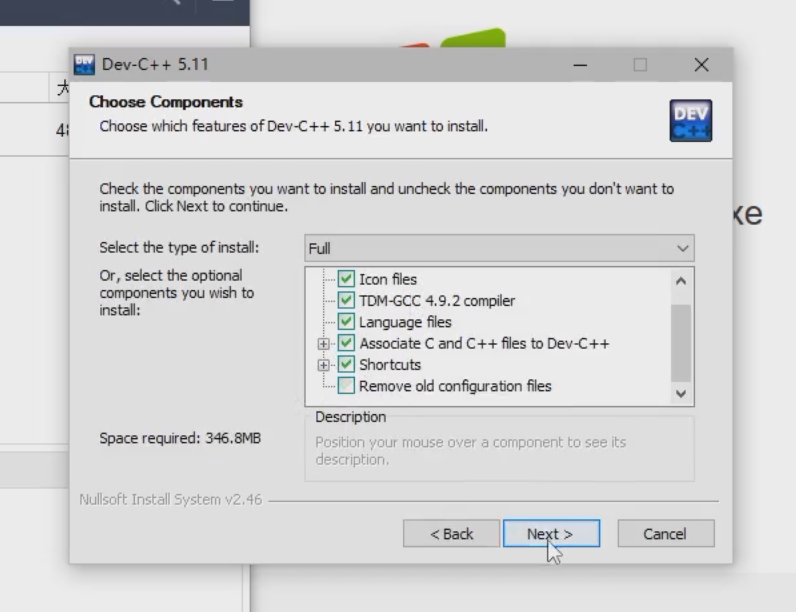
\includegraphics[width=0.6\linewidth]{01chapter/img/dev安装04}
\caption{安装组件}
\label{fig:dev04}
\end{figure}
对于安装位置,也是默认即可。
\begin{figure}[H]
\centering
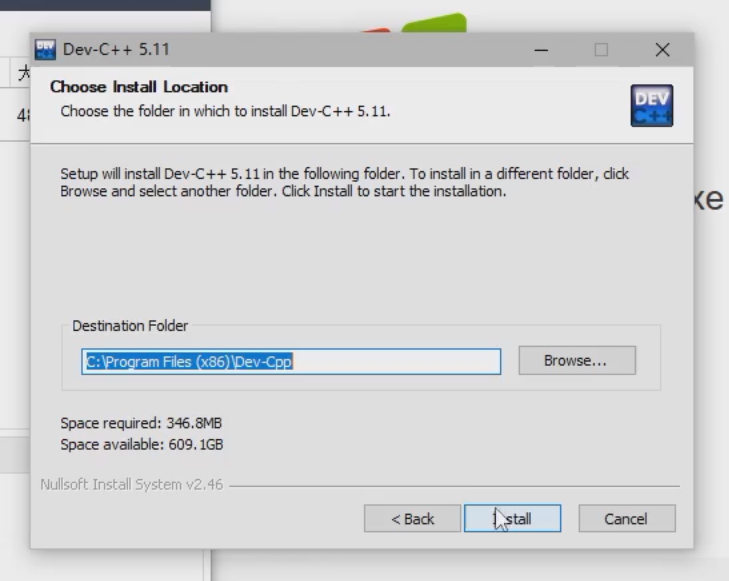
\includegraphics[width=0.6\linewidth]{01chapter/img/dev安装05}
\caption{安装位置}
\label{fig:dev05}
\end{figure}

\begin{figure}[H]
\centering
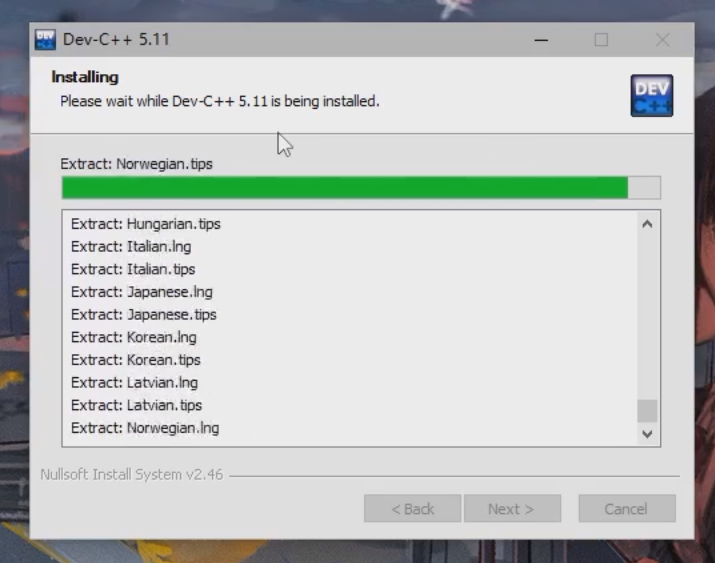
\includegraphics[width=0.6\linewidth]{01chapter/img/dev安装06}
\caption{安装过程}
\label{fig:dev06}
\end{figure}
安装结束,点击\texttt{Finish}。
\begin{figure}[H]
\centering
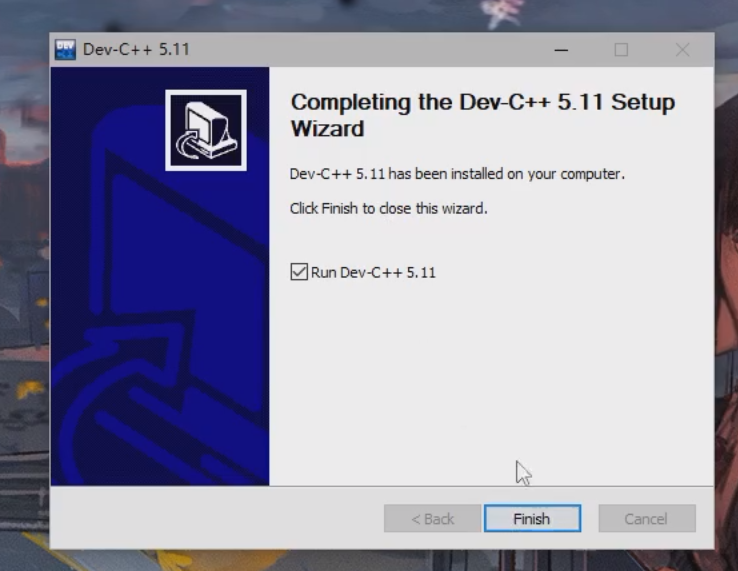
\includegraphics[width=0.6\linewidth]{01chapter/img/dev安装07}
\caption{安装结束}
\label{fig:dev07}
\end{figure}
第一次运行时,会出现语言选择部分,我们选择简体中文。
\begin{figure}[H]
\centering
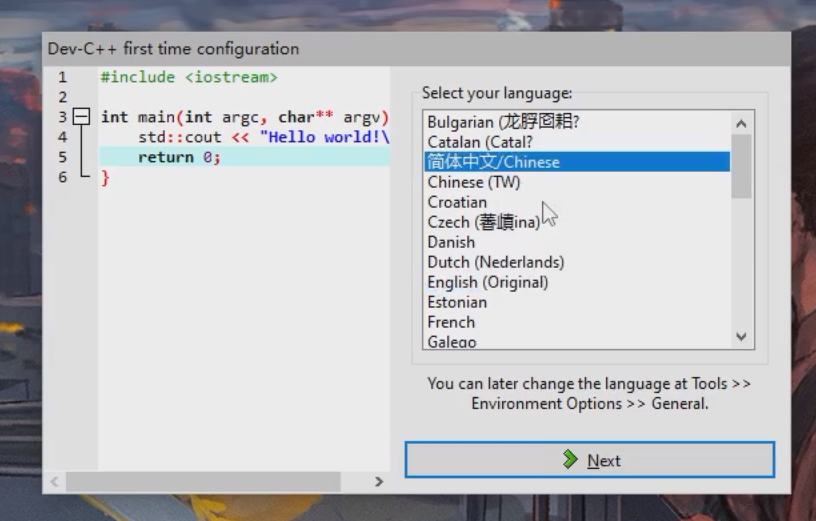
\includegraphics[width=0.6\linewidth]{01chapter/img/dev安装08}
\caption{语言选择}
\label{fig:dev08}
\end{figure}
主题部分,选默认的即可。
\begin{figure}[H]
\centering
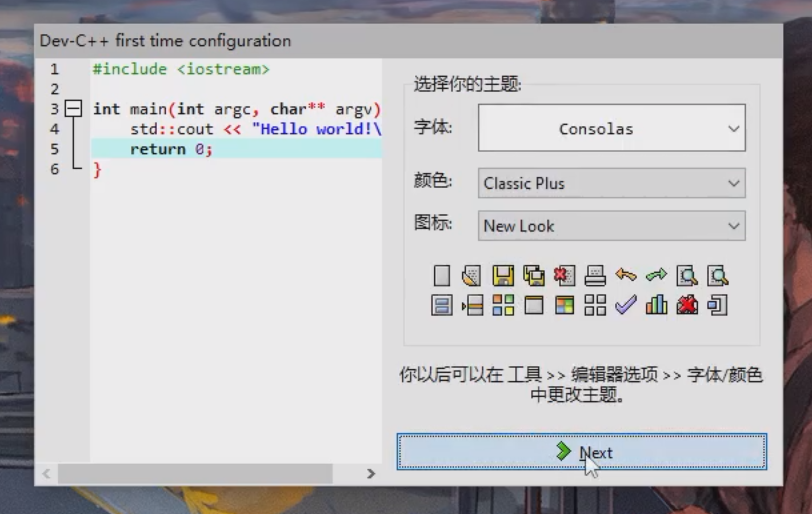
\includegraphics[width=0.6\linewidth]{01chapter/img/dev安装09}
\caption{主题选择}
\label{fig:dev09}
\end{figure}
安装完成后,我们测试下软件,看是否能正常编译运行C++程序。首先,先在软件左上角点击\texttt{文件-新建-源文件},或者是通过快捷键\texttt{Ctrl+N}的方式进行新建。
\begin{figure}[H]
\centering
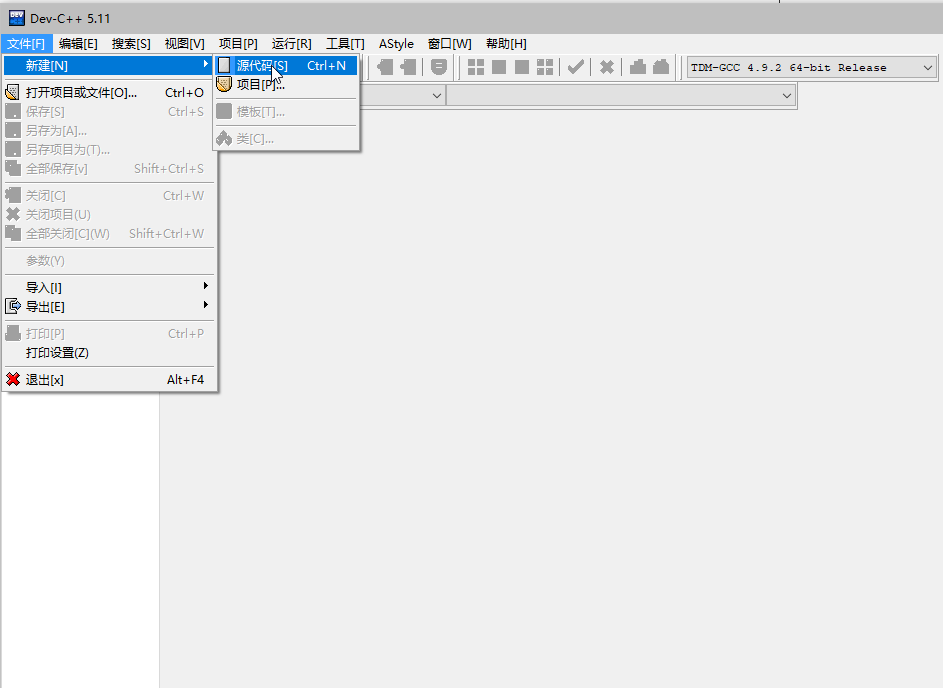
\includegraphics[width=0.6\linewidth]{01chapter/img/dev安装10}
\caption{新建源文件}
\label{fig:dev10}
\end{figure}
复制以下代码以测试程序是否能正常工作,复制粘贴完毕后,点击上方猜测方块或者是快捷键\texttt{F11}。选择好保存位置后即可编译运行。


\begin{minted}{C++}
#include <iostream>
using namespace std;
int main()
{
	cout<<"Hello world";
	return 0;
}
\end{minted}

\begin{figure}[H]
\centering
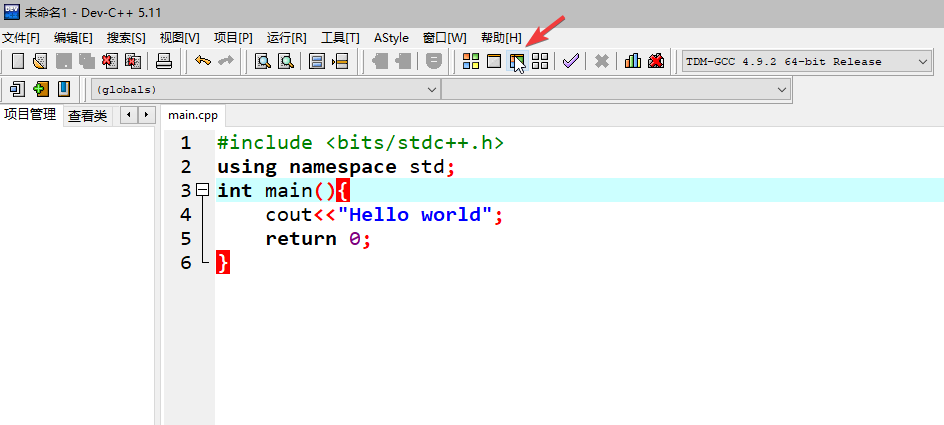
\includegraphics[width=0.6\linewidth]{01chapter/img/dev安装11}
\caption{编译运行}
\label{fig:dev11}
\end{figure}

\begin{figure}[H]
\centering
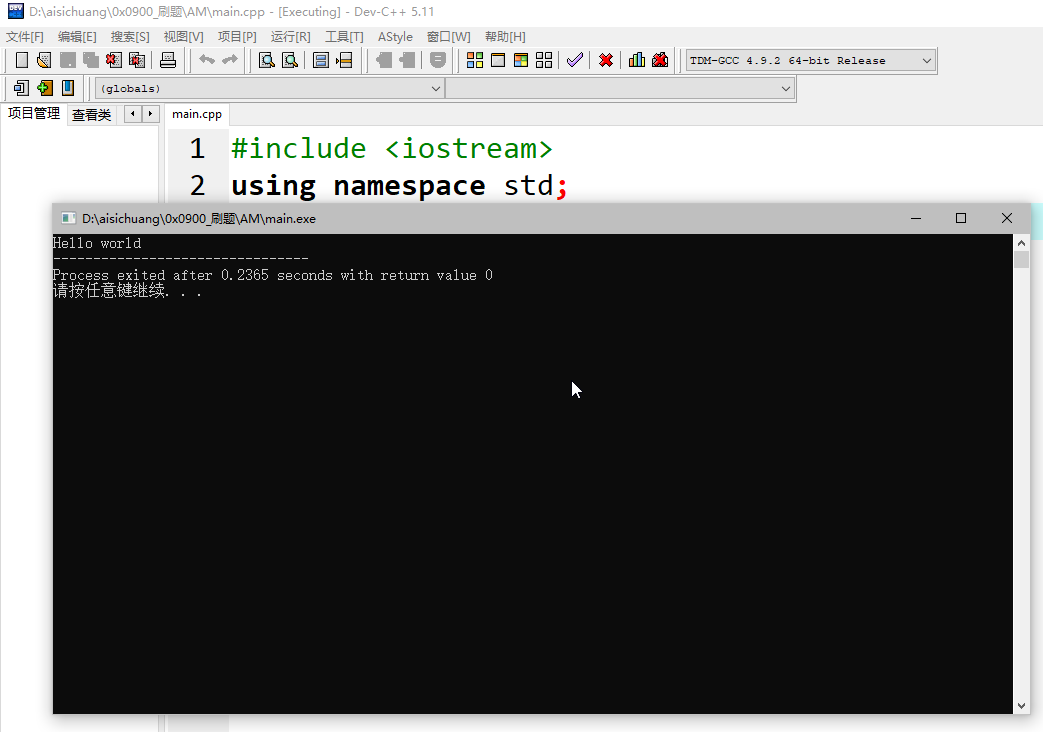
\includegraphics[width=0.6\linewidth]{01chapter/img/dev安装12}
\caption{运行结果}
\label{fig:dev12}
\end{figure}

\subsubsection{\texttt{Code::Blocks}安装}

\subsubsection{网站推荐}
推荐几个对之后的信奥大有帮助的网站,可以保存在浏览器的收藏夹中。
\begin{itemize}
\item \texttt{NOI}官网:\href{https://www.noi.cn}{https://www.noi.cn}
\item 洛谷:\href{https://www.luogu.com.cn}{https://www.luogu.com.cn}
\end{itemize}

\section{心态与方法}
“纸上得来终觉浅,绝知此事要躬行。”要将书上、课堂上的知识转化为自己的能力,需要经过大量的练习。在学习的过程中一定要注重上机实操与独立思考。对于学到的知识需要时常复习、总结。建议养成写学习博客的习惯,用自己的语言记录学习的内容。


